\documentclass[11pt]{article}

\usepackage[margin=1in]{geometry}
\usepackage{fontspec}
\usepackage{xeCJK}
\usepackage{amsmath,amssymb}
\usepackage{booktabs}
\usepackage{enumitem}
\usepackage{graphicx}
\usepackage{microtype}
\usepackage{tabularx}
\usepackage[table]{xcolor}
\usepackage[hidelinks]{hyperref}

\setCJKmainfont{Songti TC}
\setCJKsansfont{Heiti TC}
\setCJKmonofont{Heiti TC}
\xeCJKsetup{CJKecglue=\hskip 0.12em plus 0.05em minus 0.05em}

\definecolor{accent}{HTML}{315A7D}
\definecolor{lightrow}{HTML}{EEF3F7}
\setlength{\parindent}{0pt}
\setlength{\parskip}{0.55em}
\setlist[enumerate]{label=\arabic*),leftmargin=2.1em,itemsep=0.8em}
\renewcommand{\arraystretch}{1.22}
\graphicspath{{../figures/}}

\newcommand{\answer}[1]{\textcolor{accent}{\textbf{答案：}}#1}
\newcommand{\entropy}{\operatorname{H}}

\begin{document}

\section*{1. Choosing a Proximity Measure}

\begin{enumerate}
  \item \answer{Jaccard similarity。}
  將每位使用者的向量視為「曾購買商品」的集合，Jaccard similarity 定義為
  \[
    J(A,B)=\frac{|A\cap B|}{|A\cup B|}.
  \]
  兩位使用者都沒有購買的商品不會出現在聯集內，因此共同缺席不會提高相似度。
  這正符合 asymmetric binary attribute 的需求。

  \item \answer{Cosine similarity。}
  Cosine similarity 衡量兩個詞頻向量之間的夾角：
  \[
    \cos(\mathbf{x},\mathbf{y})=
    \frac{\mathbf{x}^{\mathsf T}\mathbf{y}}
         {\lVert\mathbf{x}\rVert_2\lVert\mathbf{y}\rVert_2}.
  \]
  它重視詞彙使用比例是否相近。若其中一篇文章只是整體較長，使所有詞頻同倍率增加，
  向量方向仍不變，因此相似度不受總篇幅明顯影響；此方法也適合 sparse vector。

  \item \answer{標準化後的 Euclidean distance。}
  Euclidean distance 能反映年齡、體重與醫療支出的整體幾何距離，但原始尺度差異會讓
  數值較大的醫療支出主導結果。因此，我會先以訓練資料的平均數與標準差計算
  $z$-score，再於標準化空間中計算 Euclidean distance。

  \item \answer{Pearson correlation。}
  Pearson correlation 比較中心化並標準化後的變動。較高的 baseline 會由中心化消除，
  較大的正向 amplitude 則由尺度標準化消除。因此，兩段訊號即使基準值與振幅不同，
  只要形狀及趨勢一致，相關係數仍可接近 1。
\end{enumerate}

\clearpage

\section*{2. Same Data, Different Similarity}

令
\[
 A=(5,1,5,0),\quad B=(10,2,10,0),\quad
 C=(5,5,1,5),\quad D=(1,0,1,0).
\]

\begin{enumerate}
  \item $A$ 與其他學生的 Euclidean distance 為
  \begin{align*}
    d(A,B)&=\sqrt{(5-10)^2+(1-2)^2+(5-10)^2+(0-0)^2}
           =\sqrt{51}\approx 7.141,\\
    d(A,C)&=\sqrt{(5-5)^2+(1-5)^2+(5-1)^2+(0-5)^2}
           =\sqrt{57}\approx 7.550,\\
    d(A,D)&=\sqrt{(5-1)^2+(1-0)^2+(5-1)^2+(0-0)^2}
           =\sqrt{33}\approx 5.745.
  \end{align*}
  因此，由近至遠的排序為
  \[
    \boxed{D\;\rightarrow\;B\;\rightarrow\;C}.
  \]

  \item 由向量長度與內積可得
  \begin{align*}
    \cos(A,B)&=\frac{102}{\sqrt{51}\sqrt{204}}=1.0000,\\
    \cos(A,C)&=\frac{35}{\sqrt{51}\sqrt{76}}
              =\frac{35}{\sqrt{3876}}\approx 0.5621,\\
    \cos(A,D)&=\frac{10}{\sqrt{51}\sqrt{2}}
              =\frac{10}{\sqrt{102}}\approx 0.9901.
  \end{align*}
  因此，由最相似至最不相似的排序為
  \[
    \boxed{B\;\rightarrow\;D\;\rightarrow\;C}.
  \]

  \item 兩種度量找出的最相似學生不同。Euclidean distance 選擇 $D$，因為 $D$
  的絕對活動次數較小，在數值大小上離 $A$ 最近。Cosine similarity 則選擇 $B$；
  由於 $B=2A$，兩人的活動比例與向量方向完全相同，即使 $B$ 的所有非零次數都是
  $A$ 的兩倍。前者重視絕對位移，後者重視相對活動模式。

  \item 年收入可能以數萬為單位，遠大於四個活動次數。計算原始 Euclidean distance
  時，收入差的平方可能壓過其他屬性，使結果幾乎只反映收入。我會使用訓練資料擬合
  standardization，將所有量化屬性轉為 $z$-score。若收入分布高度偏斜或含有極端值，
  也可先做 log transformation，或改用 median 與 interquartile range 的 robust scaling。
\end{enumerate}

\clearpage

\section*{3. Build a Decision Tree by Hand}

若節點中正類與負類的比例為 $p_+$ 與 $p_-$，entropy 定義為
\[
  \entropy(S)=-p_+\log_2p_+-p_-\log_2p_-,
\]
其中 $0\log_2 0$ 視為零。

\begin{enumerate}
  \item 根節點包含 $(n_+,n_-)=(3,5)$，所以
  \[
    \entropy(S)=-\frac38\log_2\frac38-\frac58\log_2\frac58
    =0.9544.
  \]

  \item 以 \emph{Height} 分割後，各子節點的類別數如下。
  \begin{center}
  \rowcolors{2}{lightrow}{white}
  \begin{tabular}{lrrrr}
    \toprule
    Height & $n_+$ & $n_-$ & Entropy & 加權貢獻 \\
    \midrule
    Short & 1 & 2 & 0.9183 & $(3/8)(0.9183)=0.3444$ \\
    Tall  & 2 & 3 & 0.9710 & $(5/8)(0.9710)=0.6068$ \\
    \bottomrule
  \end{tabular}
  \end{center}
  因此
  \[
    \entropy_{\text{Height}}=0.9512,
    \qquad \operatorname{Gain}(S,\text{Height})=0.9544-0.9512=0.0032.
  \]

  \item 以 \emph{Eyes} 分割可得
  \begin{center}
  \rowcolors{2}{lightrow}{white}
  \begin{tabular}{lrrrr}
    \toprule
    Eyes & $n_+$ & $n_-$ & Entropy & 加權貢獻 \\
    \midrule
    Brown & 0 & 3 & 0      & $(3/8)(0)=0$ \\
    Blue  & 3 & 2 & 0.9710 & $(5/8)(0.9710)=0.6068$ \\
    \bottomrule
  \end{tabular}
  \end{center}
  所以
  \[
    \entropy_{\text{Eyes}}=0.6068,
    \qquad \operatorname{Gain}(S,\text{Eyes})=0.3476.
  \]

  \item 對 nominal attribute \emph{Hair} 採用三路分割。
  \begin{center}
  \rowcolors{2}{lightrow}{white}
  \begin{tabular}{lrrrr}
    \toprule
    Hair & $n_+$ & $n_-$ & Entropy & 加權貢獻 \\
    \midrule
    Blond & 2 & 2 & 1 & $(4/8)(1)=0.5000$ \\
    Dark  & 0 & 3 & 0 & $(3/8)(0)=0$ \\
    Red   & 1 & 0 & 0 & $(1/8)(0)=0$ \\
    \bottomrule
  \end{tabular}
  \end{center}
  因此
  \[
    \entropy_{\text{Hair}}=0.5000,
    \qquad \operatorname{Gain}(S,\text{Hair})=0.4544.
  \]

  \item Hair 的 impurity reduction 最大：
  \[
  \begin{array}{c|ccc}
    \text{attribute} & \text{Height} & \text{Eyes} & \text{Hair}\\ \hline
    \text{gain} & 0.0032 & 0.3476 & \mathbf{0.4544}
  \end{array}
  \]
  因此 Hunt's algorithm 在根節點選擇 \textbf{Hair}。

  \item Dark 子節點為 $(0+,3-)$，已是純負類葉節點；Red 子節點為
  $(1+,0-)$，已是純正類葉節點。只有 Blond 子節點包含 $(2+,2-)$，
  entropy 為 1，仍需繼續分割。此節點剩餘的候選屬性如下：

  \begin{center}
  \rowcolors{2}{lightrow}{white}
  \begin{tabularx}{0.94\linewidth}{lXc}
    \toprule
    Blond 內的分割 & 子節點類別數 & 加權 entropy \\
    \midrule
    Height & Short $(1+,1-)$；Tall $(1+,1-)$
           & $(2/4)(1)+(2/4)(1)=1$ \\
    Eyes & Brown $(0+,2-)$；Blue $(2+,0-)$
         & $(2/4)(0)+(2/4)(0)=0$ \\
    \bottomrule
  \end{tabularx}
  \end{center}

  Eyes 的 gain 為 $1-0=1$，且能使兩個子節點皆為純節點。最終決策樹如下，
  每個葉節點均標示預測類別。

  \begin{center}
  \fbox{\begin{minipage}{0.70\linewidth}
  \ttfamily
  Hair?\\
  \hspace*{1.5em}|-- Dark $\longrightarrow$ 預測 $-$\\
  \hspace*{1.5em}|-- Red  $\longrightarrow$ 預測 $+$\\
  \hspace*{1.5em}`-- Blond $\longrightarrow$ Eyes?\\
  \hspace*{5.0em}|-- Brown $\longrightarrow$ 預測 $-$\\
  \hspace*{5.0em}`-- Blue  $\longrightarrow$ 預測 $+$
  \end{minipage}}
  \end{center}

  \item 將四筆測試資料套用至決策樹，可得：
  \begin{center}
  \rowcolors{2}{lightrow}{white}
  \begin{tabular}{clllcc}
    \toprule
    \# & Height & Hair & Eyes & 實際類別 & 預測類別 \\
    \midrule
    1 & Short & Dark & Brown & $+$ & $-$ \\
    2 & Short & Red  & Brown & $-$ & $+$ \\
    3 & Short & Red  & Blue  & $+$ & $+$ \\
    4 & Tall  & Red  & Brown & $+$ & $+$ \\
    \bottomrule
  \end{tabular}
  \end{center}
  四筆資料中有兩筆預測正確，因此
  \[
    \text{accuracy}=\frac24=0.50=50\%,\qquad
    \text{error rate}=1-0.50=0.50=50\%.
  \]
\end{enumerate}

\clearpage

\section*{4. Mini Lab - Similarity Meets Classification}

資料切分採用 0.25 的 test fraction、
random state 42 與 stratification；所有模型均為最大深度 3、random state 2 的
decision tree。

\begin{enumerate}
  \item Iris 資料集共有 150 筆資料與 4 個輸入特徵。類別名稱為 setosa、
  versicolor 與 virginica，各有 50 筆。切分所用的 random state 為 42，
  切分後有 112 筆訓練資料與 38 筆測試資料。

  \item StandardScaler 僅使用 112 筆訓練資料進行擬合，再分別轉換訓練集與測試集。
  兩個模型的比較如下。

  \begin{center}
  \small
  \rowcolors{2}{lightrow}{white}
  \begin{tabular}{lllll}
    \toprule
    模型 & 根節點分割 & 葉節點 & 訓練準確率 & 測試準確率 \\
    \midrule
    原始資料 & petal width $\leq 0.8000$ cm & 5 & 0.9821 & 0.9211 \\
    標準化資料 & standardized petal width $\leq -0.5135$ & 5 & 0.9821 & 0.9211 \\
    \bottomrule
  \end{tabular}
  \end{center}

  兩棵樹的深度皆為 3，分支結構也相同。原始單位下，規則分別在 petal width
  的 0.80 與 1.70 cm，以及 petal length 的 4.95 與 4.85 cm 進行分割；
  標準化後相對應的門檻變為 $-0.51$、0.66、0.67 與 0.61。兩個模型對 38 筆
  測試資料的預測完全相同。

  標準化只改變門檻的數值座標，不會改變單一特徵內各觀測值的排序。Decision tree
  每次只在一個特徵上尋找切點，因此候選分割仍然相同。Euclidean distance 則會把
  不同特徵的座標差合併計算；改變任一特徵的尺度，就會改變該特徵對總距離的貢獻，
  進而可能改變 nearest neighbors。

  \item 原始 decision tree 的 training accuracy 為 0.9821，test accuracy
  為 0.9211。這個差距表示模型在未見資料上的表現略有下降。若 training accuracy
  遠高於 test accuracy，通常代表 overfitting：模型學到了訓練資料中的偶然邊界或
  雜訊，卻無法推廣至新資料。可透過限制深度、pruning，或利用驗證資料選擇
  hyperparameters 來改善。

  \item 由原始訓練集以 random state 42 抽取 stratified subsets，並保持測試集不變。

  \begin{center}
  \small
  \rowcolors{2}{lightrow}{white}
  \begin{tabular}{rrrrrr}
    \toprule
    比例 & 訓練筆數 & 根節點特徵 & 門檻 & 深度 / 葉節點 & 測試準確率 \\
    \midrule
    20\%  & 22  & Petal width & 0.80 & 3 / 4 & 0.9211 \\
    40\%  & 44  & Petal width & 0.70 & 3 / 4 & 0.9211 \\
    60\%  & 67  & Petal width & 0.70 & 3 / 4 & 0.9737 \\
    80\%  & 89  & Petal width & 0.80 & 3 / 5 & 0.9211 \\
    100\% & 112 & Petal width & 0.80 & 3 / 5 & 0.9211 \\
    \bottomrule
  \end{tabular}
  \end{center}

  所有訓練資料量下，第一個分割特徵皆為 petal width，但門檻會在 0.70 與
  0.80 cm 之間變動。樹深固定為允許的最大值 3，葉節點數則在 80\% 時由 4 增為 5。
  測試準確率大多維持 0.9211，只有 60\% 的子集達到 0.9737。因此，增加訓練資料
  並不保證決策樹會更深或準確率會單調提高。不同樣本可能改變 impurity-optimal
  threshold 與下層分支，而固定的 depth limit 也限制了模型複雜度。

  \begin{figure}[ht]
    \centering
    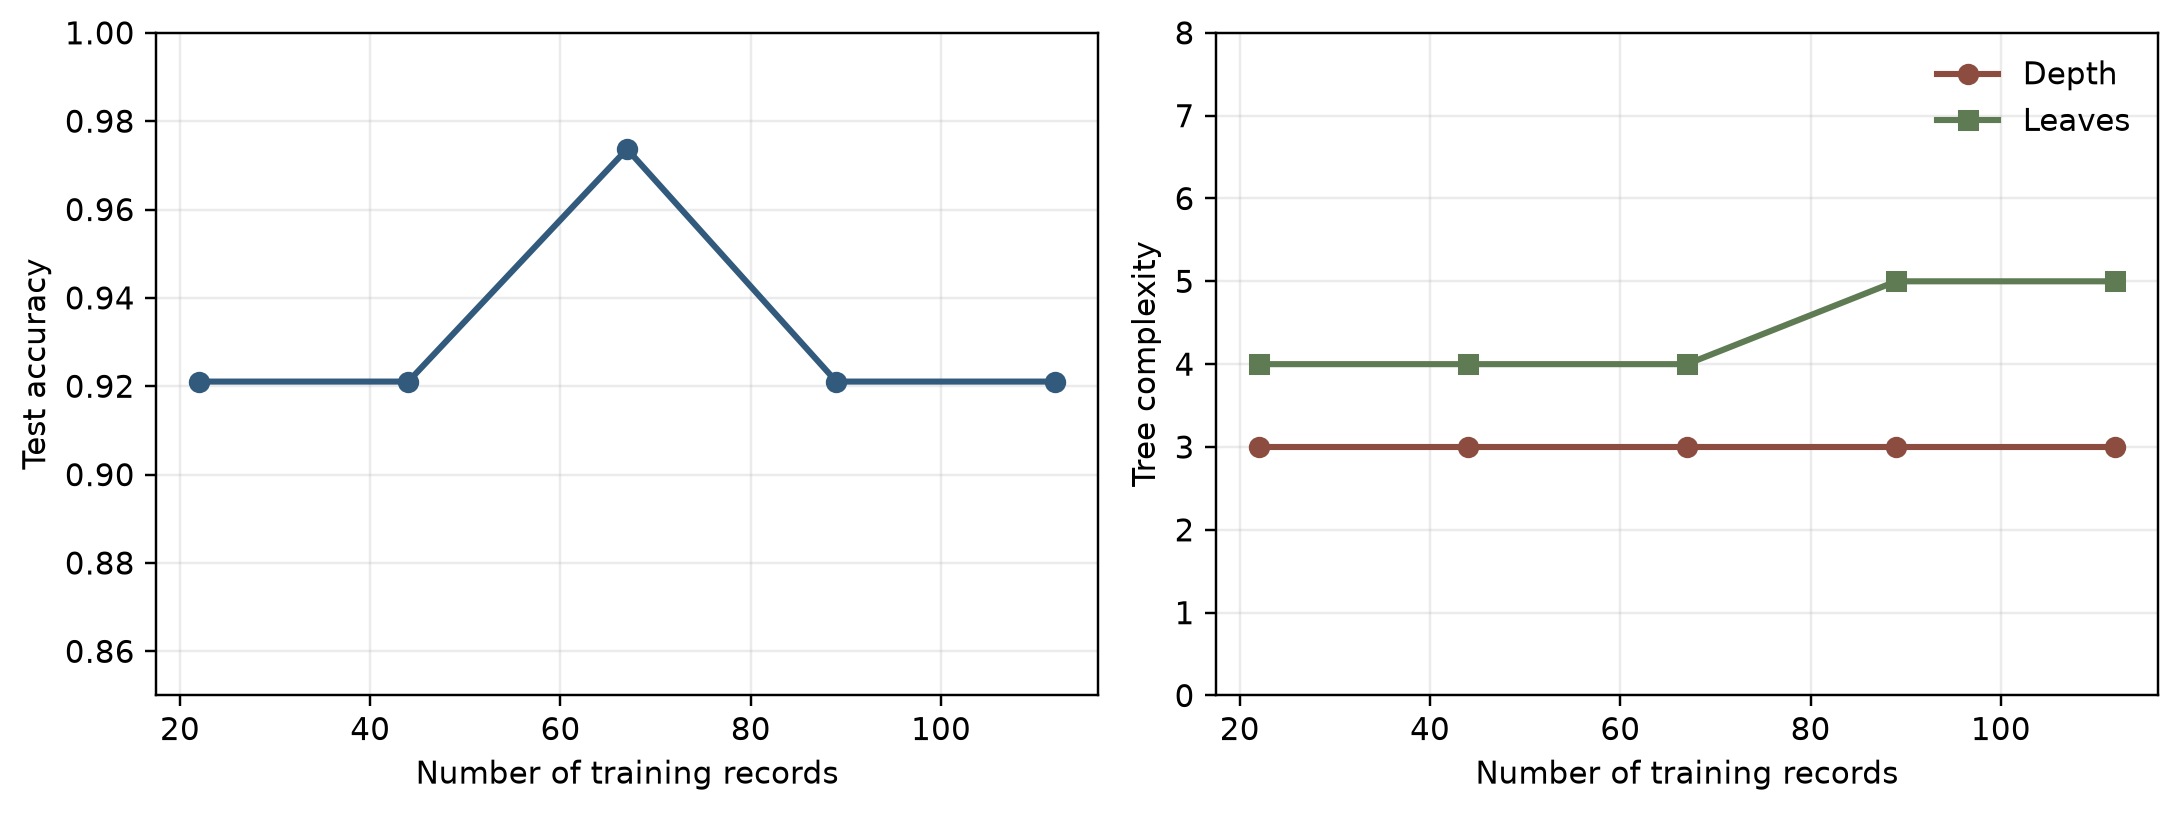
\includegraphics[width=0.94\linewidth]{q4_training_size.png}
    \caption{固定測試集下，訓練資料量、測試準確率與決策樹複雜度的關係。}
  \end{figure}

  \item \textbf{綜合說明（內容對應英文版 131 words）。}
  標準化改變了分割門檻的數值，卻沒有改變 decision tree 所選的特徵、資料分區、
  預測結果或準確率。這與 axis-aligned tree 的運作方式一致：單調的尺度轉換會保留
  特徵內部的數值順序。Euclidean-distance neighbors 的情況不同，因為特徵尺度會
  直接改變合併後的距離。原始模型的訓練準確率為 0.982、測試準確率為 0.921，
  兩者只有小幅 generalization gap；若差距很大，才較可能表示 overfitting。
  在不同大小的 stratified training subsets 中，petal width 始終是根節點特徵，
  但門檻與葉節點數會改變。測試準確率在 60\% 訓練資料時最高，之後又回到原來水準。
  因此，更多資料不一定單調增加樹深或準確率；sampling variation 會改變最佳分割，
  固定的 depth limit 則會限制模型複雜度。
\end{enumerate}


\section*{Generative AI disclosure}
本報告使用 OpenAI Codex 協助整理分析架構、撰寫 Python實驗，以及進行 LaTeX 排版。

\end{document}
